\documentclass[12pt, oneside]{amsart}
\usepackage[margin=1in]{geometry}                % See geometry.pdf to learn the layout options. There are lots.
\geometry{letterpaper}                   % ... or a4paper or a5paper or ... 
\usepackage[parfill]{parskip}        % Begin paragraphs with an empty line rather than an indent
\usepackage{graphicx}
\usepackage{amssymb}
\usepackage{epstopdf}
\usepackage{url}
\usepackage[comma,authoryear]{natbib}
\DeclareGraphicsRule{.tif}{png}{.png}{`convert #1 `dirname #1`/`basename #1 .tif`.png}

% Different font in captions
\newcommand{\captionfonts}{\small}

\makeatletter  % Allow the use of @ in command names
\long\def\@makecaption#1#2{%
  \vskip\abovecaptionskip
  \sbox\@tempboxa{{\captionfonts #1: #2}}%
  \ifdim \wd\@tempboxa >\hsize
    {\captionfonts #1: #2\par}
  \else
    \hbox to\hsize{\hfil\box\@tempboxa\hfil}%
  \fi
  \vskip\belowcaptionskip}
\makeatother   % Cancel the effect of \makeatletter

% My contribution is:  What am I doing, how is it unique, what are the steps.

\title{An Open Model for Climate Behaviors}
\author{James Rising}

\begin{document}
\maketitle

% FUTURE CONSIDERATIONS (on next print!)
% Refer to transport several times as case study/application
% Hierarchy of Models, Held '05 (from IPCC)
% Notes from transit speaker
% Ostrom's variables (A General Framework for Analyzing Sustainability of Social-Ecological Systems) (SES) - framework for cumulation

The goal of the Open Model for Climate Behaviors is to identify drivers and leverage points in the social system surrounding climate change, by developing new approaches in system modeling and analysis.  The project combines system dynamics with spatial and network methods, uniquely building on the strengths of each, and synthesizing a wide range of models and data.  This framework has wide applicability, and the first case study will focus on passenger transportation behaviors in the United States.  By identifying underlying forces in coupled social, economic, and political systems, this research can help focus research and facilitate effective policymaking.  The spatially explicit and institutionally specific results are simultaneously accessible to scientists and the public, helping bridge divisions between these groups.

Anthropomorphic climate change and environmental degradation are among the most pressing issues of our time, and despite a recent explosion of green technologies and strategies, the social behaviors that drive climate change remain intractable.  Politicians, businesses, and consumers may individually favor changes, but mutually reinforcing incentives make action difficult or costly.  This kind of overdetermined homeostasis is typical of complex systems.  While the feedback loops that support the status quo reduce the effectiveness of some actions, whether they are new laws, citizen movements, or business decisions, other changes can be reinforced and amplified.  These ``leverage points'' are places where small changes can make pervasive differences.  Due to the structural nature of complex systems, from ecosystems to economies, leverage points are ubiquitous, if difficult to identify \citep{meadows1997places}.  To better understand the dense network of social realities that affect behaviors surrounding climate change, this research aims to develop a high-dimensional numerical model, along with the tools to elucidate it.

Passenger transportation offers an ideal example.  Transportation is the second largest and fastest growing source of U.S. greenhouse gas emissions and passenger cars produce the largest portion of US transportation emissions.  Models suggest that changes in development patterns and transport behaviors can reduce vehicle travel by 10-25\% while improving accessibility \citep{greene2011reducing}.  However, many factors reinforce a culture of driving, from a lack of public transportation to suburban layouts.  As a result, where driving is the norm some changes, like improving public transit options and supporting services close to homes, can have a high cost and little benefit.  Identifying the right entry point is key to developing effective policies.  Modeling the wider system of relevant factors, from the cost of cars the frequency of rain, can lead to policies that benefit all parties, while leveraging a greater effect on emissions.  

The coupling of human and natural systems results in new layers of complexity, which have only recently begun to be explored \citep{liu2007complexity}.  This emerging research can benefit from a new modeling framework which applies the temporal sophistication of system dynamics to the spatial heterogeneity typical of coupled systems.  It provides the greatest advantage for problems that are currently intractable due to an overdetermined set of reinforcing drives, and that are spatially heterogeneous.  A wide range of environmental and public health issues fit this description.  Examples include environmental degradation, agricultural practices in poor countries, obesity, substance abuse, groundwater use, and fishery management, as well as situations fraught with rebound effects \cite[as in][]{greening2000energy} and environmental standards that shift activity across borders (e.g., carbon leakage).


The strengths of Columbia's PhD in Sustainable Development support this work, with the rigor of its economic foundations, the strong foundation it provides in the natural and human sciences, and the many opportunities provided under the Earth Institute and the Center for Research on Environmental Decisions (CRED) Lab.  Material from this research will form the basis for the author's dissertation on the opportunities for society to adapt to the new demands of a climate-strained world.  With the aid of the EPA's support and feedback, this new framework has the potential to dramatically improve our capacity to model large, heterogeneous systems, to understand the complex roles of existing institutions in influencing our climate behaviors, and to integrate a wide variety of models and make them accessible to policymakers.
%Tackling environmental problems that have complex, distributed social drivers requires new tools like the Open Model for performing integrated analysis.
\section*{Methodology}

The Open Model for Climate Behaviors combines four fundamental components to better identify leverage points: (1) support for multiple network maps and conditional self-similarity, (2) integration of time series data, (3) computational tools for model evaluation, and (4) an open interface for contributions and communication.  Each component builds on a variety of prior work, but their combination is one this project's significant contributions.

A wide range of models have been developed to understand pro-environmental behavior and how to motivate it \citep{kollmuss2002mind, Hines1986}.  This `agency' approach has uncovered a variety of social forces, but scaling individual behaviors to society wide dynamics has proven difficult \citep{may1954intransitivity}.  In the case of transportation, \citet{redclift1994social} note,
\begin{quotation}
\begin{small}
The great majority of individuals may be `locked into' patterns of daily activity (such as private car use) which they know to be environmentally destructive.  Only if the spatial separations of work, shopping, leisure and residence were changed, or if public investment into socialized transport provision were greatly increased and transformed would individuals have a meaningful \emph{choice} to make about transport options for themselves.
\end{small}
\end{quotation}

This research applies the insights and techniques of system dynamics, founded in Forrester's work in organizational dynamics \citeyearpar{forrester1961industrial} and Meadows et al's \emph{Limits to Growth} \citeyearpar{meadows2004limits}.  Of the many fields used to model the factors that influence our habits, from community psychology to economics, system dynamics offers a number of advantages exploited by this work.  System dynamics explicitly (and visually) describes feedback loops and policy conditions, which allows researchers and policymakers to experiment with policy changes and illustrate the results.  It provides results than can be interpreted both quantitatively (for verification) and qualitatively (with reference to established small-model behaviors like those from \citet{senge2006fifth}).  Finally, existing models, such as the World3/2000 model used by \citeauthor{meadows2004limits} and Forrester's urban dynamics model, are available as a baseline.  The techniques of system dynamics have been applied to many sectors relevant to this project, including urban growth and decline \citep{forrester1971urban}, energy policy \citep{Naill1992}, environment management \citep{fletcher1998use, Guo2001}, public health \citep{Homer2001}, and social change initiatives \citep{repenning2002simulation}.\footnote{For an introduction to the tools and methodologies of system dynamics, see \cite{sterman2000business} for model-making, \cite{senge2006fifth} for intuition, and \cite{meadows1997places} for leverage points.}

One weakness of system dynamics is that it is hugely aggregative.  In traditional system models, distinguishing even between demographic populations requires reproducing all of the relevant relations influencing them both, as well the dynamics between them.  In addition, system models handle space poorly, tending to treat a distributed stock, such as arable land, as a single lump sum.

\cite{ahmad2004spatial} addresses this by integrating geographic information system modeling (GIS) and system dynamics, calling the approach spatial system dynamics (see figure A).  This technique has been used for flood management \citep{ahmad2006intelligent}, water resource modeling \citep{vivoni2009semiarid, roach2009compartmental}, and invasive species spread \citep{bendor2006spatial}.
\begin{figure}[tb]
\begin{tabular}{ccc}
  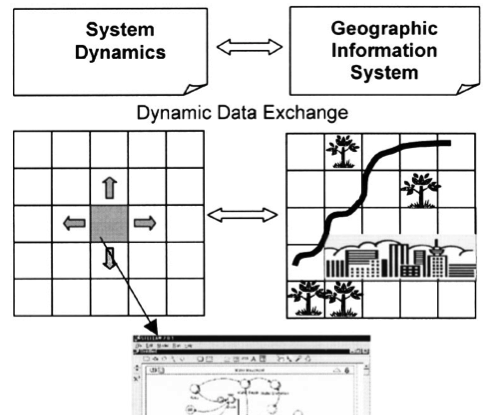
\includegraphics[width=2in]{ssdarch-mod2.png} & 
  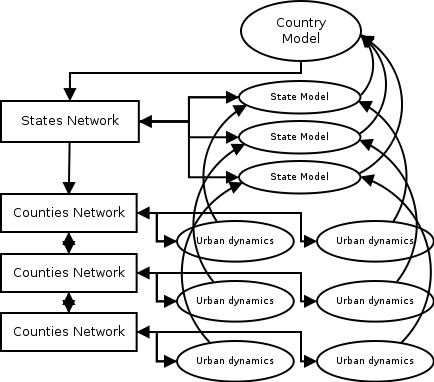
\includegraphics[width=2in]{architecture.png} &
  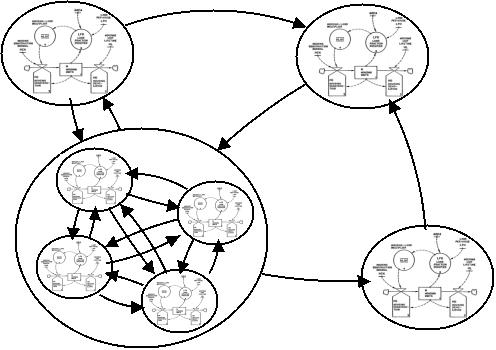
\includegraphics[width=2in]{selfsimodel.jpeg} \\
  \parbox[t]{2in}{(A) {\bf Architecture of the spatial system dynamics approach}, modified from \cite{ahmad2004spatial}.  System dynamics handles temporal modeling, which the parameters of each cell are provided by GIS data.} &
  \parbox[t]{2in}{(B) {\bf Partial architecture of the full model}.  Aggregate dynamics from the Country Model are distributed through the States Network to each state's model.  The State Models also relays stocks through the States Network.} &
  \parbox[t]{2in}{(C) {\bf Self-similarity and drilling-down with system dynamics}.  Each region is represented as a node, and each node may be associated with a further division of the region with another network.}
\end{tabular}
\end{figure}

This project extends spatial system dynamics into a powerful network-based approach with models that can vary between regions.  This provides three advantages.  First, it allows different networks for different dynamics.  For example, a grid network is appropriate for modeling climate change, but the road network better represents how people travel.  This project pioneers the use of multiple networks to represent the different ways stocks flow between nodes (e.g. across land or along roads), demographic groups, and institutional relations (see figure B).\footnote{The author has analyzed Internal Revenue Service migration data and airline flight prices to form potential networks.}  Second, the use of networks helps capture the self-similarity common to social systems.  Many social systems exhibit the small-world property \citep{watts1998collective}, scale-free behavior \citep{barabasi1999emergence}, and hierarchical modularity \citep{ravasz2002hierarchical}, which are naturally expressed through network structures.  Third, the networks can form a hierarchy of scales, which allow a new kind of fractal analysis.  Global dynamics will be modeled with global parameters, but with the potential to ``drill down'' to arbitrary levels of detail, allowing the model to function on a sufficiently fine-grain to identify the particular institutions at the heart of leverage points (see figure C).\footnote{Within climate prediction research, the process of moving between resolution scales is called downscaling, and that literature informs this process \citep{murphy1999evaluation}.}

In traditional system models, time series data are only used for parameter tuning and model verification \citep{Forrester1991}.  In this framework, data has a more complementary role, driving both the downscaling (drilling-down) process, defining the pattern of spatial heterogeneity, and supporting the computational identification of missing or contradictory relationships.  A variety of techniques exist to validate system dynamical models \citep{barlas1996formal, graham1976parameter}, and this project adapts them to larger a computation framework.  However, like traditional system dynamic models and unlike climate models, the purpose of the Open Model is to capture the dynamics implicit in institutional relationships and not to predict future states.

In additional to developing tools to validate inter-model dynamics, the project involves the creation of a variety of tools necessary to run experiments and interpret the underlying drivers of the results.  In particular, these tools will identify key elements, relationships, and loops which can significantly effect the dynamics of the whole system.  Following \cite{meadows1997places}, the system will analyze changes in parameters, buffer sizes and flow speeds, the strength of feedback loops, and the structure of information flows to seek potential points of leverage.

Finally, the Open Model will be open: it will include an online interface for other researchers to make contributions and analyze the results.  By connecting with other scientists on the Internet, the project becomes both more manageable and more useful.\footnote{Group model building is widely used in system dynamics both for education and as a tool for creating accurate models \citep{rouwette2002group}.}  As a platform for researches to run their partial models within a larger context, this framework can help to identify both strengths and contradictions between existing models.  Different researchers can identify drivers for different outcome variables, such as CO$_2$ emissions, the well-being populations, and the biodiversity of ecosystems.

\section*{Implementation Details}
\label{sec:implementing}

The process for pursuing this research follows five overlapping phases: additional research, framework implementation, model development, analysis, and policy recommendations.  Many of the core framework elements are already complete and in use for the author's current research on flooding and self-organized economies.  These elements include a basic synthesis of system dynamics and multiple network maps, some integration with time series data, and a growing set of tools for analysis.

As a first application, the Open Model will be applied to passenger driving behaviors.  It will include the policies, businesses, materials, environment, and political economy surrounding and influencing the actions of American drivers.  It is difficult to estimate the number of system elements necessary to support the search for leverage points.  Nation-wide models range in side considerably, from 283 variables for World3/2000 to over 2000 in the System Dynamics National Model.  The monumental \emph{Encyclopedia of World Problems and Human Potential} has identified 56,135 ``problems,'' ranging from ``loss of cultural diversity'' to ``youth gangs'', and identified within them 2,675 environmental feedback loops, ``problems that are implicated in many negative feedback systems concerning the natural environment'' \citep{ewphp}.

Actual changes in climate may also have a strong effect on behavior, so climate prediction must inform the model as a whole.  Initially, the model can use pre-computed results from climate models, but climate change represents a coupled natural and human system.  Incorporating a general climate model (GCM) into this framework presents a considerable computation challenge, but few conceptual difficulties.

The Open Model project envisions an evolving dialogue with policymakers and institutional actors, as a boundary-bridging knowledge system \citep{cash2003knowledge}.  The first step of this process is to conduct interviews with the relevant stakeholders and institutions, to supplement a literature review in understanding the interconnections behind current behaviors.  This has been found to be both an effective way to collect the necessary information, and a beneficial exercise for stakeholders to better understand the system within which they work \citep{rouwette2002group}.  System dynamical models are ideal for communcation and accessibility, both because of their intuitive structure and their support for active learning \citep{senge2006fifth}.  These actors will be invited to maintain an active role in reviewing and advising the model as it develops.

This research has a considerable potential to inform policy decisions concerning the difficult problems of climate change and environmental damage.  Using an open interface for contributions, review, and analysis, this model can also provide a powerful framework for integrating existing knowledge and uncovering new knowledge through innumerable experiments.  The model also encourages communication with and participation of the general public and diverse groups, easily providing results catered to them.

The complexity of the social, political, and economic system surrounding climate change requires new tools, drawing on the strengths of many fields.  The modeling framework described represents not just an expansion or knitting together of existing models, but a unique construct which elegantly draws on the strengths of these different techniques.  By combining system dynamics, networks, self-similarity, time series data, and computational analysis, this framework can capture the dynamics of social systems on a finer scale than previously possible.  With the help of the EPA, this new model can provide considerable benefits to both researchers and policymakers.

\newpage
\bibliography{openmodel}{}
\bibliographystyle{apalike}

\end{document}

